\documentclass[tikz,border=5pt]{standalone}
\usetikzlibrary{positioning}
\begin{document}
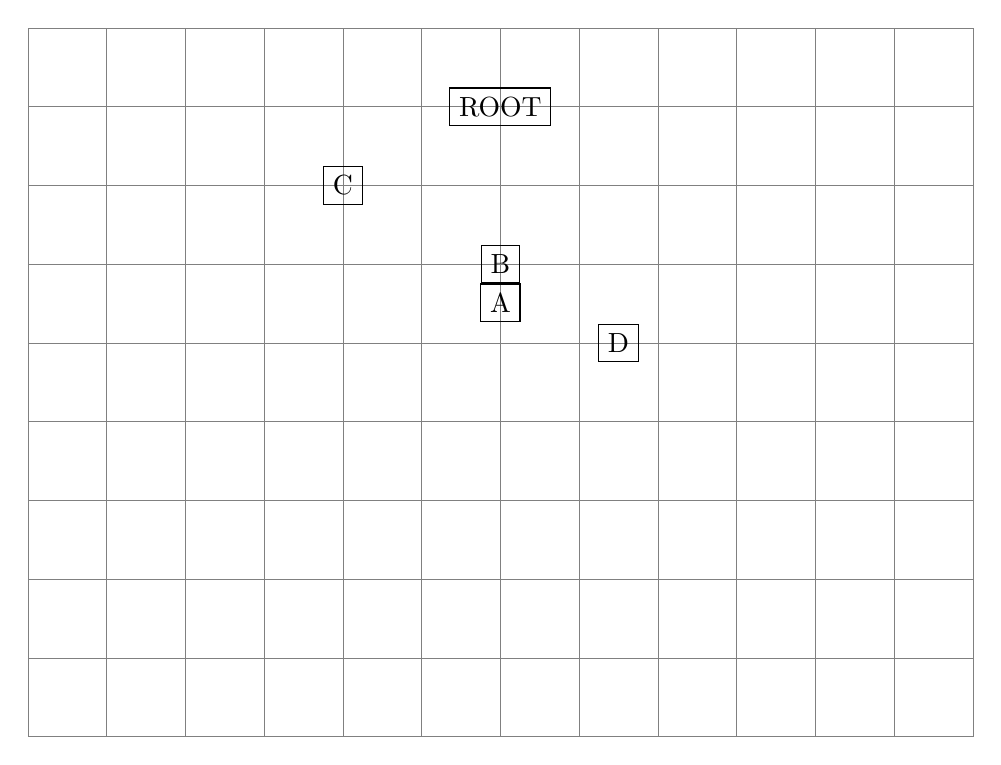
\begin{tikzpicture}[every node/.style={draw}]
\draw[help lines,step=1cm] (-6,1) grid (6,-8);
\node (root) {ROOT};
\node[below=2cm of root] (A) {A};%
\node[on grid,below=2cm of root] (B) {B};
\node[on grid,below left=1cm and 2cm of root] (C) {C};
\node[on grid,below right=3cm and 1.5cm of root] (D) {D};
\end{tikzpicture}
\end{document}